\documentclass[a4paper,11pt,english]{article}
\usepackage{hyperref}
\usepackage{stmaryrd,palatino, url, multicol,graphicx,float,color}
\usepackage[margin=3cm]{geometry}
\usepackage[bottom]{footmisc}
\usepackage{psfrag}
\usepackage{listings}
\lstset{
%	backgroundcolor=\color{none},
	basicstyle=\footnotesize,
	tabsize=4,
	rulecolor=,
	language=java
}	
\usepackage{color}
\begin{document}
\title{High Scalable Scientific Computing using Hadoop}
\author{Ing. Jos\'e Pablo Alberto Andreotti, Lic. Nicol\'as Wolovick, Dr. Javier Blanco.}
%TODO:Nico, c�mo meto los mails ac�??? 
\date{Famaf. Diciembre de 2010.}
\maketitle
\begin{abstract}

This work provides a description of our experience in trying to apply
the capabilities of Hadoop\cite{HadoopSite}
to scientific problems. Hadoop is a
framework intended to provide open-source software for reliable, 
scalable, and distributed computing. It is the opensource 
counterpart of Google's map-reduce framework. Hadoop is often applied
to data mining problems, in which large amounts of data\footnote{Even reaching the order of petabytes.} 
in the form of strings are processed.\\

On the other hand, scientific applications work mostly on binary data
that is stored in structures such as arrays or matrixes. Our intention
is to leverage Hadoop capabilities such as scalability, fault tolerance,
and load balancing, in order to target scientific workloads.
We describe our experience by discussing a specific example application
that solves the problem of heat transfer in a squared board.\\
\\
\end{abstract}
\section{Introduction to Hadoop}
Hadoop is a framework intended to provide open-source software for reliable, 
scalable, and distributed computing. Support for Reliability comes into play with
the use of commodity hardware where failures chances are high.
Map-reduce is a \emph{linearly scalable} programming model that works on a distributed set of
machines. The programmer writes two functions, a \emph{map function} and a \emph{reduce function}.
\\
Furthermore, Hadoop is the opensource counterpart of Google's
map-reduce framework. Hadoop is often applied to data mining problems, in which 
large amounts of data in the form of strings are processed. The most widely known
parts of Hadoop are the map-reduce framework and
the HDFS distributed filesystem. We will explain the concepts associated with
them in the following sections.\\
\subsection{Map-Reduce}
The basic idea behind the map-reduce model of computation is to divide 
the computation into two phases: \emph{map} and \emph{reduce}. Input data is first 
processed by the map phase, whose output data will be the input to the
reduce phase. The reduce phase will produce the final output. Both the
input and output of the map and reduce functions is in the $(key, value)$ format.\smallskip \\
During the map phase, multiple map functions begin execution. The number
of these functions is determined by how the input data is processed. Input data is composed by
a number of $(key, value)$ pairs. As it will be explained later, Hadoop provides
a \emph{serialization framework} to work with data in this format.\\
All values sharing the same key will be given
as input to the same map function, and the number of map functions will be 
equal to the number of unique keys in the input data.\\
In a similar fashion, multiple reduce functions begin execution during the 
reduce phase. The mission of the reduce functions is to take the output of
the map phase and write the final output to disk. An example of this model
can be seen in Figure \ref{fig:map_red}.\\
The input to the map functions is taken from the HDFS file system. Then
the output of these functions is sorted, and is provided as input to the
reduce phase. In this example only two distinct keys are present at the
output of the map phase, thus only two reduce functions are spawned.
As we will show later, more complex computations may include a succession
of multiple map-reduce cycles.\\


\begin{figure}[H]
\begin{center}
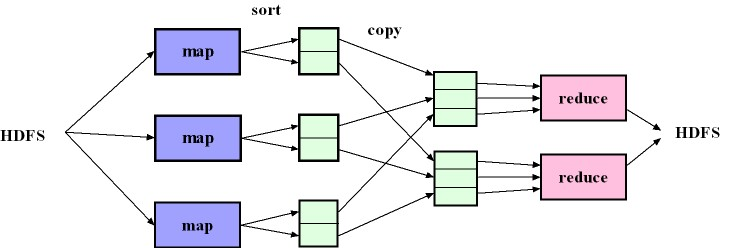
\includegraphics[hiresbb=false,bb= 0 0 272mm 85mm, scale=0.57, 
clip=true,keepaspectratio=true]
{map_red.jpg}
\caption{\label{fig:map_red}\footnotesize
Example of a map-reduce job with three maps and two reduces.
}
\end{center}
\end{figure}
\subsection{HDFS}
As we have previously discussed, Hadoop is intended to handle very large amounts of data,
i.e., thousands of Gigabytes. The Hadoop Distributed Filesystem (HDFS)
is designed to store these data reliably, and to stream them to applications at high bandwidth. 
In this section, we will briefly explain the architecture of HDFS. The explanation will 
reproduce some of the paragraphs found in \cite{HDFSPaper}. However, for the sake of brevity,
much of the material found in this paper was omitted, so we encourage the reader to take
a look at the full paper for a complete description.
\smallskip\\
HDFS stores file system metadata and application data separately. More specifically, HDFS
stores metadata on a dedicated server, called the \emph{NameNode}. Application data is stored on
other servers called \emph{DataNodes}. All servers are fully connected and communicate with each 
other using TCP-based protocols. Reliability is achieved by replicating file contents on 
multiple DataNodes.\\
In this way, not only data reliability such as in RAid is assured, but also this strategy has
the added advantage that data transfer bandwidth is multiplied, and there are more opportunities
for locating computation \emph{near} the needed data. \\
The basic architecture consists in a NameNode, DataNodes and HDFS Clients.
The NameNode stores the HDFS namespace which is a hierarchy of files and directories.
Files and directories are represented on the NameNode by inodes, which record attributes like 
permissions, modification and access times, namespace and disk space quotas. The file
content is split into large blocks (typically 128 megabytes) and each block of the file is 
independently replicated at multiple DataNodes (typically three). The NameNode maintains the
namespace tree and the mapping of file blocks to DataNodes. \\
An HDFS client wanting to read a
file first contacts the NameNode for the locations of data blocks comprising the file and
then reads block contents from the closest DataNode. 
When writing data, the client requests the NameNode to nominate a suite of three
DataNodes to host the block replicas. The client then writes data to the DataNodes in a pipelined
fashion. \\
Each block replica on a DataNode is represented by two files in the local host's native file 
system. The first file contains the data itself and the second file is block's metadata including
checksums for the block data and the block�s generation stamp. During startup each DataNode 
connects to the NameNode and performs a handshake. The purpose of the handshake is to
verify the \emph{namespace id} and the software version of the DataNode. If either does not match
that of the NameNode, the DataNode automatically shuts down. The namespace id identifies all
the nodes that belong to the filesystem instance. The consistency of software versions is 
important because incompatible version may cause data corruption or loss.\\
After the handshake, the DataNode registers with the NameNode. DataNodes persistently store
their unique storage ids. The storage id is an internal identifier of the DataNode,
which makes it recognizable even if it is restarted with a different IP address or port.
The storage id is assigned to the DataNode when it registers with the NameNode for the first
time and never changes after that. During normal operation DataNodes send \emph{heartbeats} to the
NameNode to confirm that the DataNode is operating and the block replicas it hosts are available.
The NameNode does not directly call DataNodes. Instead, it uses replies to heartbeats to send instructions
to the DataNodes.\\
The last part we will discuss is the HDFS client.
The HDFS filesystem interface
is accessed by user applications by means of a library. The user references files and directories
by paths in the namespace, and can perform the typical read, write and delete operations in a way
that is very similar to UNIX filesystems. The user generally does not need to know that file system
metadata and storage are on different servers, or that blocks have multiple replicas.\\
\begin{figure}[H]
\begin{center}
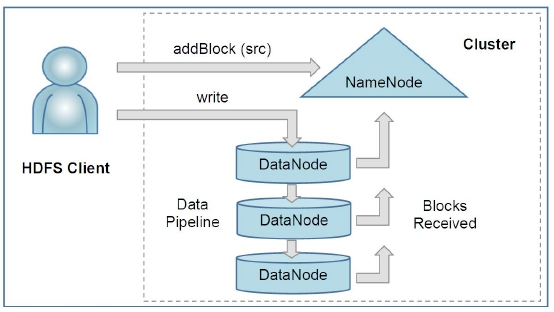
\includegraphics[hiresbb=false,bb= 0 0 201mm 111mm, scale=0.47, 
clip=true,keepaspectratio=true]
{HDFS_arch.jpg}
\caption{\label{fig:hdfs_arch}\footnotesize
An HDFS client creates a new file by giving its path to the NameNode. For each block of the file,
the NameNode returns a list of DataNodes to host its replicas. The client then pipelines data to 
the chosen DataNodes, which eventually confirm the creation of the block replicas to the NameNode.
This figure was taken from \cite{HDFSPaper}.
}
\end{center}
\end{figure}
When an application reads a file, the HDFS client first asks the NameNode for the list of DataNodes
that host replicas of the blocks of the file. It then contacts a DataNode directly and requests the
transfer of the desired block. When a client writes, it first asks the NameNode to choose DataNodes
to host replicas of the first block of the file. The client organizes a pipeline from node-to-node
and sends the data. When the first block is filled, the client requests new DataNodes to be chosen
to host replicas of the next block. A new pipeline is organized, and the client sends the further 
bytes of the file. Each choice of DataNodes is likely to be different. The interactions among the
client, the NameNode and the DataNodes are illustrated in Figure \ref{fig:hdfs_arch}.


\subsection{Jobs}
%A job in Hadoop is the smallest unit of work that can be scheduled.
A user provides a Job to the framework in order to execute useful work. A summary of the 
interaction of a user defined Job and the framework is provided in Table \ref{table:hadoop_parts},
which was extracted from \cite{ProHadoop}.
\smallskip \\
First, the user configures a job specifying the input and its location, and ensures the input is
in the expected format, and then submits the job to the framework. The job is also configured
with a map and a reduce function. The framework then decomposes this job into a set of map tasks,
shuffles, a sort, and a set of reduce tasks. \\
After that, the framework fragments the data and distributes it among the nodes in the cluster, which 
can in turn be provided as input to the individual distributed tasks. Each fragment of input is
called an \emph{input split}.\\

\begin{table}[ht]
\caption{Parts of a Hadoop Job} % title of Table
\centering 
\begin{tabular}{l l}
\hline \hline 
Part & Handled by \\ [0.5ex]
\hline \small
Configuration of the Job. & User \\[0.65ex]
Input splitting and distribution. & Hadoop framework\\[0.65ex]
Start of the individual map tasks with their input split. & Hadoop framework\\[0.65ex]
Map function, called once for each input key/value pair. & User\\[0.65ex]
Shuffle, which partitions and sorts the per-map output. & Hadoop framework\\[0.65ex]
Sort, which merge sorts the shuffle output for each partition & Hadoop framework\\
of all map outputs.\\[0.65ex]
Start of the individual reduce tasks, with their input partition. & Hadoop framework\\[0.65ex]
Reduce function, which is called once for each input key, & User\\
with all of the input values that share that key.\\[0.65ex]
Collection of the output and storage in the configured job output& Hadoop framework\\
directory, in N parts, where N is the number of reduce tasks.\\[0.65ex]
\hline \hline 
\end{tabular}
\label{table:hadoop_parts}
\end{table}

The framework will then distribute and start the execution of the tasks, with their input splits.
Job management is handled by two processes that are provided by the framework,
\begin{itemize}
\item TaskTracker: manages the execution of individual map and reduce tasks on a compute
node in the cluster.
\item JobTracker: accepts job submissions, provides job monitoring and control, and manages
the distribution of tasks to the TaskTracker nodes.
\end{itemize}
Generally, there is one JobTracker process per cluster and one or more TaskTracker processes
per node in the cluster. The framework is responsible for distributing the job among the TaskTracker
nodes of the cluster; running the map, shuffle, sort, and reduce phases; placing the output in the
output directory; and informing the user of the job-completion status.\\

\subsection{The Serialization Framework}

Serialization is the process of turning structured objects into a byte stream for transmission
over a network or for writing to persistent storage. Deserialization is the reverse
process of turning a byte stream back into a series of structured objects.\smallskip \\
Serialization appears in two quite distinct areas of distributed data processing: for
interprocess communication and for persistent storage.
In Hadoop, interprocess communication between nodes in the system is implemented
using remote procedure calls (RPCs). The RPC protocol uses serialization to render the
message into a binary stream to be sent to the remote node, which then deserializes the
binary stream into the original message. \\
%In general, it is desirable that an RPC serialization
%format is:
%Compact
%A compact format makes the best use of network bandwidth, which is the most
%scarce resource in a data center.
%Fast
%Interprocess communication forms the backbone for a distributed system, so it is
%essential that there is as little performance overhead as possible for the serialization
%and deserialization process.
%Extensible
%Protocols change over time to meet new requirements, so it should be
%straightforward to evolve the protocol in a controlled manner for clients and servers.
%For example, it should be possible to add a new argument to a method call,
%and have the new servers accept messages in the old format (without the new argument)
%from old clients.
%Interoperable
%For some systems, it is desirable to be able to support clients that are written in
%different languages to the server, so the format needs to be designed to make this
%possible.
The data format chosen for persistent storage would have different
requirements from a serialization framework. After all, the lifespan of an RPC is less
than a second, whereas persistent data may be read years after it was written. As it turns
out, the desirable properties of an RPC�s serialization format are also crucial for a
persistent storage format. \\
Hadoop uses its own serialization format, \emph{Writables}, which is certainly compact and
fast, but not so easy to extend or use from languages other than Java. Since Writables
are central to Hadoop (most MapReduce programs use them for their key and value
types), we will focus on them.\\
\subsubsection{The Writable Interface}
The Writable interface defines two methods: one for \emph{writing} its state to a DataOutput
binary stream, and one for \emph{reading} its state from a DataInput binary stream:

\begin{figure}[H]
\begin{center}
\begin{lstlisting}
package org.apache.hadoop.io;
import java.io.DataOutput;
import java.io.DataInput;
import java.io.IOException;

public interface Writable {
    void write(DataOutput out) throws IOException;
    void readFields(DataInput in) throws IOException;
}
\end{lstlisting}
\caption{\label{list:red_fine}\footnotesize
The Writable Interface.}%
\end{center}
\end{figure}

As an example of a writable, we will use IntWritable, a wrapper for a Java int. We can
create one and set its value using the set() method: \\

\begin{figure}[H]
\begin{center}
\begin{lstlisting}
IntWritable writable = new IntWritable();
writable.set(163);
\end{lstlisting}
\caption{\label{list:red_fine}\footnotesize
Basic usage of IntWritable.}%
\end{center}
\end{figure}
Objects that implement the Writable interface can be used to form the splits provided 
as input to the map and reduce functions.
\section{Heat Transfer Problem}
\subsection{Description of the problem}
The problem we are dealing with is a classical problem of heat transfer in
a squared area. The problem is solved by finding a solution for Laplace's equation,\\ \\
\begin{center}
\LARGE
$\frac{\partial^2 \Phi }{\partial^2 x} + \frac{\partial^2 \Phi}{\partial^2 y} = 0$ \\ \\
\normalsize
\end{center}
Where $\Phi$ is the unknown scalar potential that represents the heat at each point.
%The method we are using is an \emph{stencil computation}. 
In this heat transfer model, a squared surface with side length L is divided into a mesh,
and each cell within the mesh is assigned an initial temperature value.The objective is
to approximate the steady-state solution for points within the mesh.

The Jacobi iteration is a common iterative method used to solve Laplace's equation. We will
use the Jacobi iteration to solve the equation and will base our explanation and pseudocode
on the description found in \ref{}.
Then, the temperature of each cell at time $t+1$ is computed averaging the temperature
of the neighbouring cells at time at time $t$. 
The zoomed area of Figure \ref{fig:problem_div} explains how this division is performed, 
and the resulting neighbours for a sample cell $h_{ij}$.
Figure \ref{fig:problem_comp} explains how this computation takes place for a sample cell.\\
\begin{figure}[H]
\begin{center}
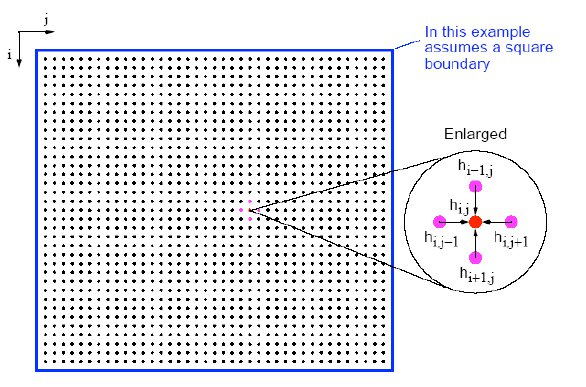
\includegraphics[hiresbb=false,bb= 0 0 201mm 141mm, scale=0.47, 
clip=true,keepaspectratio=true]
{problem_desc.jpg}
\caption{\label{fig:problem_div}\footnotesize
The squared area is divided into a mesh.
}
\end{center}
\end{figure}

\begin{figure}[H]
\begin{center}
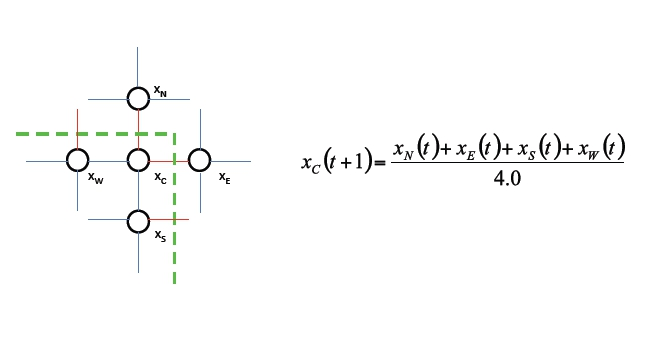
\includegraphics[hiresbb=false,bb= 0 0 241mm 101mm, scale=0.47, 
clip=true,keepaspectratio=true]
{problem_comp.jpg}
\caption{\label{fig:problem_comp}\footnotesize
Each cell's temperature on the next step is calculated by averaging the temperature of its
neighbours.
}
\end{center}
\end{figure}

Finally in Figure \ref{fig:problem_sample} an example is provided where four steps of
the computation can be seen for some sample data.

\begin{figure}[H]
\begin{center}
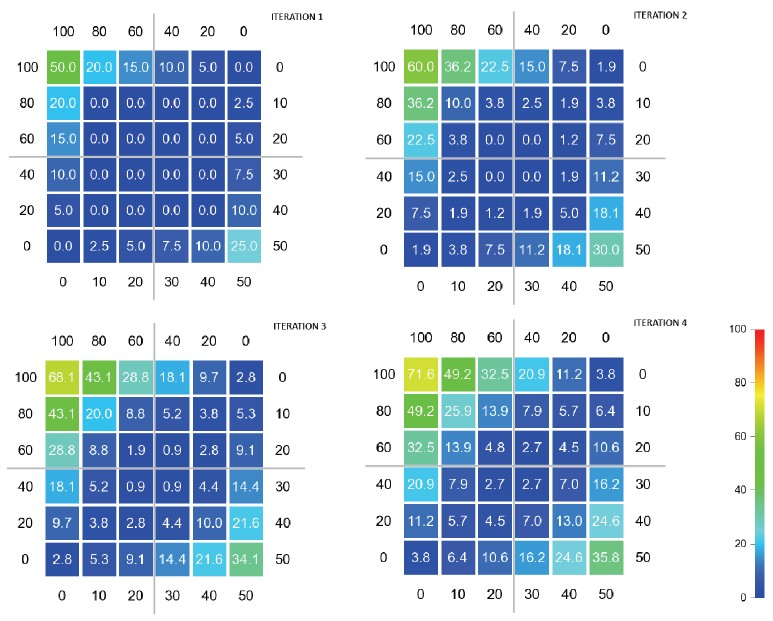
\includegraphics[hiresbb=false,bb= 0 0 278mm 221mm, scale=0.45, 
clip=true,keepaspectratio=true]
{problem_sample.jpg}
\caption{\label{fig:problem_sample}\footnotesize
Four iterations of the Stencil's aproximation are shown. The values next to the borders
are heat sources at fixed temperatures.
}
\end{center}
\end{figure}


\subsubsection{Convergence}
This calculation of temperatures based on the previous state of the neighbouring cells takes place
until certain convergence criteria is met. To explain this, suppose that an initial state of the 
surface included a heat source in certain cell. The temperature of this cell will remain the same
during the whole computation.\smallskip \\
As one may suspect, it may come a point where all the cells surrounding the heat source will be at
about the same temperature of the heat source, and eventually the whole surface will be at the same
temperature of the heat source. This is what will match our physical intuition, and we will expect
the model to behave in this way, but we are really more interested in studying how the heat flows
in a point at time that is before that obvious limit.\\
In order to accomplish that, we will consider that the simulation has \emph{converged} when the 
difference between each of the $h_{ij}$ cells in two successive steps of the computation is less
than certain value $C$ which we will choose conveniently.

\subsubsection{Translating into a map-reduce application}
The challenge when writing a map-reduce application is to Figure out how the computation will
be organized in a set of map and reduce tasks, and how these tasks are fed with the input data. 
We will explore two alternative approaches to achieve this in the next Section.


\subsection{First Alternative}
The first option we will consider is to have a map function that distributes 
each individual element of the matrix to all its neighbours. Thus, if after 
the execution of all the map functions, all the
neighbours of any element i are sent to reduce function i, the calculation
can take place on the reduce function.\\
In this way, the information that is output from the map phase is \emph{four times} 
the size of the original input information. This implies, that we will have a network
traffic that is four times the size of the input data. Furthermore, we will have
$LxL$ map functions and $LxL$ reduce functions. In the next section we will explore an
alternative solution that tries to reduce the overhead from both sources. We will have 
a performance comparison in section \ref{sec:performance}.

In order to achieve this distribution of data, the input data must be stored
in a way by which every single element in the matrix is given as input to a 
single unique map function. We do this by storing each matrix element with its
own key, being the key the linear position of the element in the matrix. This is
shown in Figure \ref{fig:serialization}.\\

\begin{figure}[H]
\begin{center}
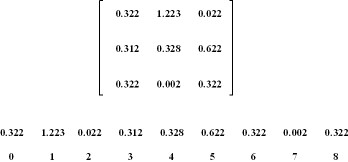
\includegraphics[hiresbb=false,bb= 0 0 131mm 57mm, scale=0.77, 
clip=true,keepaspectratio=true]
{serialization.jpg}
\caption{\label{fig:serialization}\footnotesize
The matrix is stored as a succession of (key, value) pairs being each key an 
IntWritable and each value a FloatWritable.
}
\end{center}
\end{figure}

\begin{figure}[H]
\begin{center}
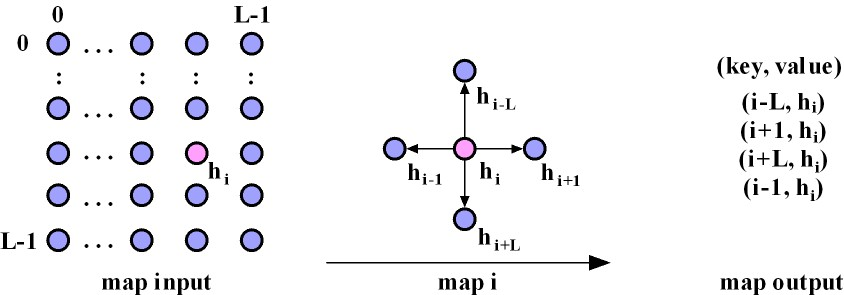
\includegraphics[hiresbb=false,bb= 0 0 300mm 111mm, scale=0.37, 
clip=true,keepaspectratio=true]
{map_fine.jpg}
\caption{\label{fig:map_fine}\footnotesize
Map function for our first solution of the heat transfer problem.
}
\end{center}
\end{figure}
The resulting map function that process this input data can be seen in Figure \ref{fig:map_fine}.
On the left we have
the input data. In the middle, we have the map function that distributes each element to
all its neighbouring cells. The right part shows the output of the map function, which is
a set of $(key,value)$ pairs.\\
The matching reduce function is in Figure \ref{fig:red_fine}. On the left,
there is the input data, in the $(key, value)$ form. In the middle, we see how each reduce function
receives as its input the temperature values of its neighbouring cells during the last step. On the
right side of the figure is the output data. Each reduce function contributes to a single element
in the output data.\\
The listings for the map and reduce, can be seen in Figure \ref{list:map_fine}, and Figure
 \ref{list:red_fine}, respectively.\\

\begin{figure}[H]
\begin{center}
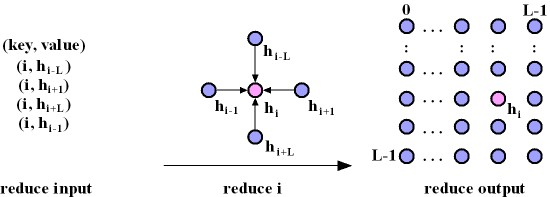
\includegraphics[hiresbb=false,bb= 0 0 208mm 68.5mm, scale=0.55, 
clip=true,keepaspectratio=true]
{red_fine.jpg}
\caption{\label{fig:red_fine}\footnotesize
Reduce function for our first alternative solution of the heat transfer problem. 
}
\end{center}
\end{figure}


\begin{figure}[H]
\begin{center}
\begin{lstlisting}
public class HeatTransfer {

    public static class TokenizerMapper
    extends Mapper<IntWritable, FloatWritable, IntWritable, FloatWritable>{

    public void map(IntWritable key, FloatWritable fwValue, Context context
                            ) throws IOException, InterruptedException {
       int myKey = key.get();
       
       //Distribute my value to the previous and the next
	   key.set(myKey - 1);
       context.write(key, fwValue);
       key.set(myKey + 1);
       context.write(key, fwValue);

       //Distribute my value to the cells above and below
       key.set(myKey - MatrixData.Length());
       context.write(key, fwValue);
       key.set(myKey + MatrixData.Length());
       context.write(key, fwValue);

    }//end map
  }//TokenizerMapper
}//HeatTransfer

\end{lstlisting}
\caption{\label{list:map_fine}\footnotesize
Map function implementing the behaviour of Figure \ref{fig:map_fine}. In this listing,
the method MatrixData.Length() correspond to the length of the matrix, L.}%
\end{center}
\end{figure}

\begin{figure}[H]
\begin{center}
\begin{lstlisting}
public class HeatTransfer {

     public void reduce(IntWritable key, Iterable<FloatWritable> fwValues, 
                       Context context) throws IOException, InterruptedException {

       float result = 0.0f;
       
       //Handle first and last "cold" boundaries
       if(key.get()<0 || key.get()>MatrixData.LinearSize()){
          return;
       }
       
	   //Keep the heat source
       if(key.get()==MatrixData.HeatSourceLinearPos()){
          context.write(key, new FloatWritable(MatrixData.HeatSourceTemperature()));
          return;
       }

       //Add all the values
       for(FloatWritable fw : fwValues) {
          result += fw.get();
       }
       
      context.write(key, new FloatWritable(result/4) );

    }//end reduce
}//end HeatTransfer
\end{lstlisting}
\caption{\label{list:red_fine}\footnotesize
Reduce function implementing the behaviour of Figure \ref{fig:red_fine}.}%
\end{center}
\end{figure}


\subsection{Second Alternative}
The next option we are exploring distributes data with a grosser granularity pattern.
Instead of distributing each individual element, the map functions will now distribute
entire rows of the matrix. The key to be used will be the row number within the matrix.
This map function is depicted in Figure \ref{fig:map_gross}.Similarly, the reduce function now will take three rows as input. This is shown
in Figure \ref{fig:red_gross}. 

\begin{figure}[H]
\begin{center}
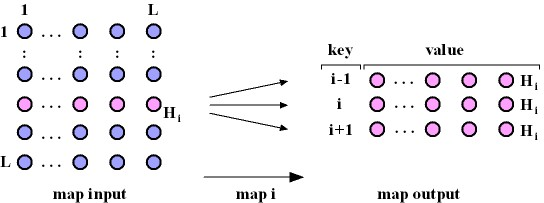
\includegraphics[hiresbb=false,bb= 0 0 201mm 72mm, scale=0.53, 
clip=true,keepaspectratio=true]
{map_gross.jpg}
\caption{\label{fig:map_gross}\footnotesize
Map function for our second alternative solution of the heat transfer problem.
}
\end{center}
\end{figure}

Now every reduce function will have three rows as input, and these will be used to perform
the computation of a whole output row. 

\begin{figure}[H]
\begin{center}
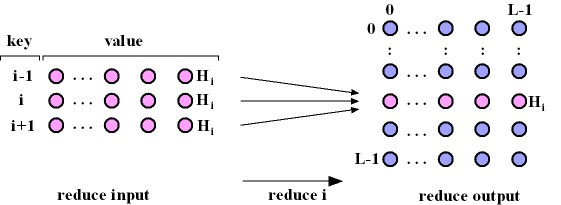
\includegraphics[hiresbb=false,bb= 0 0 201mm 72mm, scale=0.54, 
clip=true,keepaspectratio=true]
{red_gross.jpg}
\caption{\label{fig:red_gross}\footnotesize
Reduce function for our second alternative solution of the heat transfer problem.
}
\end{center}
\end{figure}



%GnuPlot Commands: 
%set terminal postscript eps rounded enhanced color
%set output '2dplot.eps'
%set label 'n' at 10700000,1300
%set grid 10000, 13000
%show grid
%plot  "perf.dat" using 1:2 title 'Fine' with linespoints, \
%      "perf.dat" using 1:3 title 'Gross' with linespoints


\section{Performance}
\label{sec:performance}
Now that we have an interesting problem in place with two alternative solutions, we
would like to explore how the framework is doing regarding scalability. For doing 
this we decided to run the application in a different number of nodes.

    \begin{figure}[H]
%     \psfrag{eq}[b]{$\displaystyle\frac{v + W}{ v + W/n}$}
%     \psfrag{asym}{$S_{max} = 1 + W/v$}
%	  \psfrag{n}[b]{$n$ {\footnotesize(n\'umero de procesadores)}}
	  \begin {center}
      \includegraphics{2dplot.eps}
	  \end{center}
	  \caption{\footnotesize
       This graph depicts how both implementations perform for a fixed size problem of
	   $N=12.000$. The applications were run in one, two, four and eights processors.
      }
    \end{figure}


\begin{thebibliography}{2}
\bibitem{HadoopSite} Hadoop website http://hadoop.apache.org/.
\bibitem{HDFSPaper} The Hadoop Distributed File System, Konstantin Shvachko,
Hairong Kuang, Sanjay Radia, and Robert Chansler (Proceedings of MSST2010, May 2010, available at \href{http://
storageconference.org/2010/Papers/MSST/Shvachko.pdf}{http://storageconference.org/2010/Papers/MSST/Shvachko.pdf}).
\bibitem{ProHadoop} Pro Hadoop, Jason Venner, Apress 2009.
\end{thebibliography}
	
	
\section{Appendix A: Description of the Java code.}	
Here are the listings of the two implementations for the example studied. 

\section{Appendix B: Configuration of the Hadoop environment.}	
Here are the listings of the two implementations for the example studied. 

%FIGURES

\end{document}
